\yesmargins

\chapter{Paper Prototyping\index{paper prototype}}

\begin{tikzpicture}[overlay,remember picture] 
\node[anchor=south] at ([yshift=5in,xshift=0.8in]current page text area.south){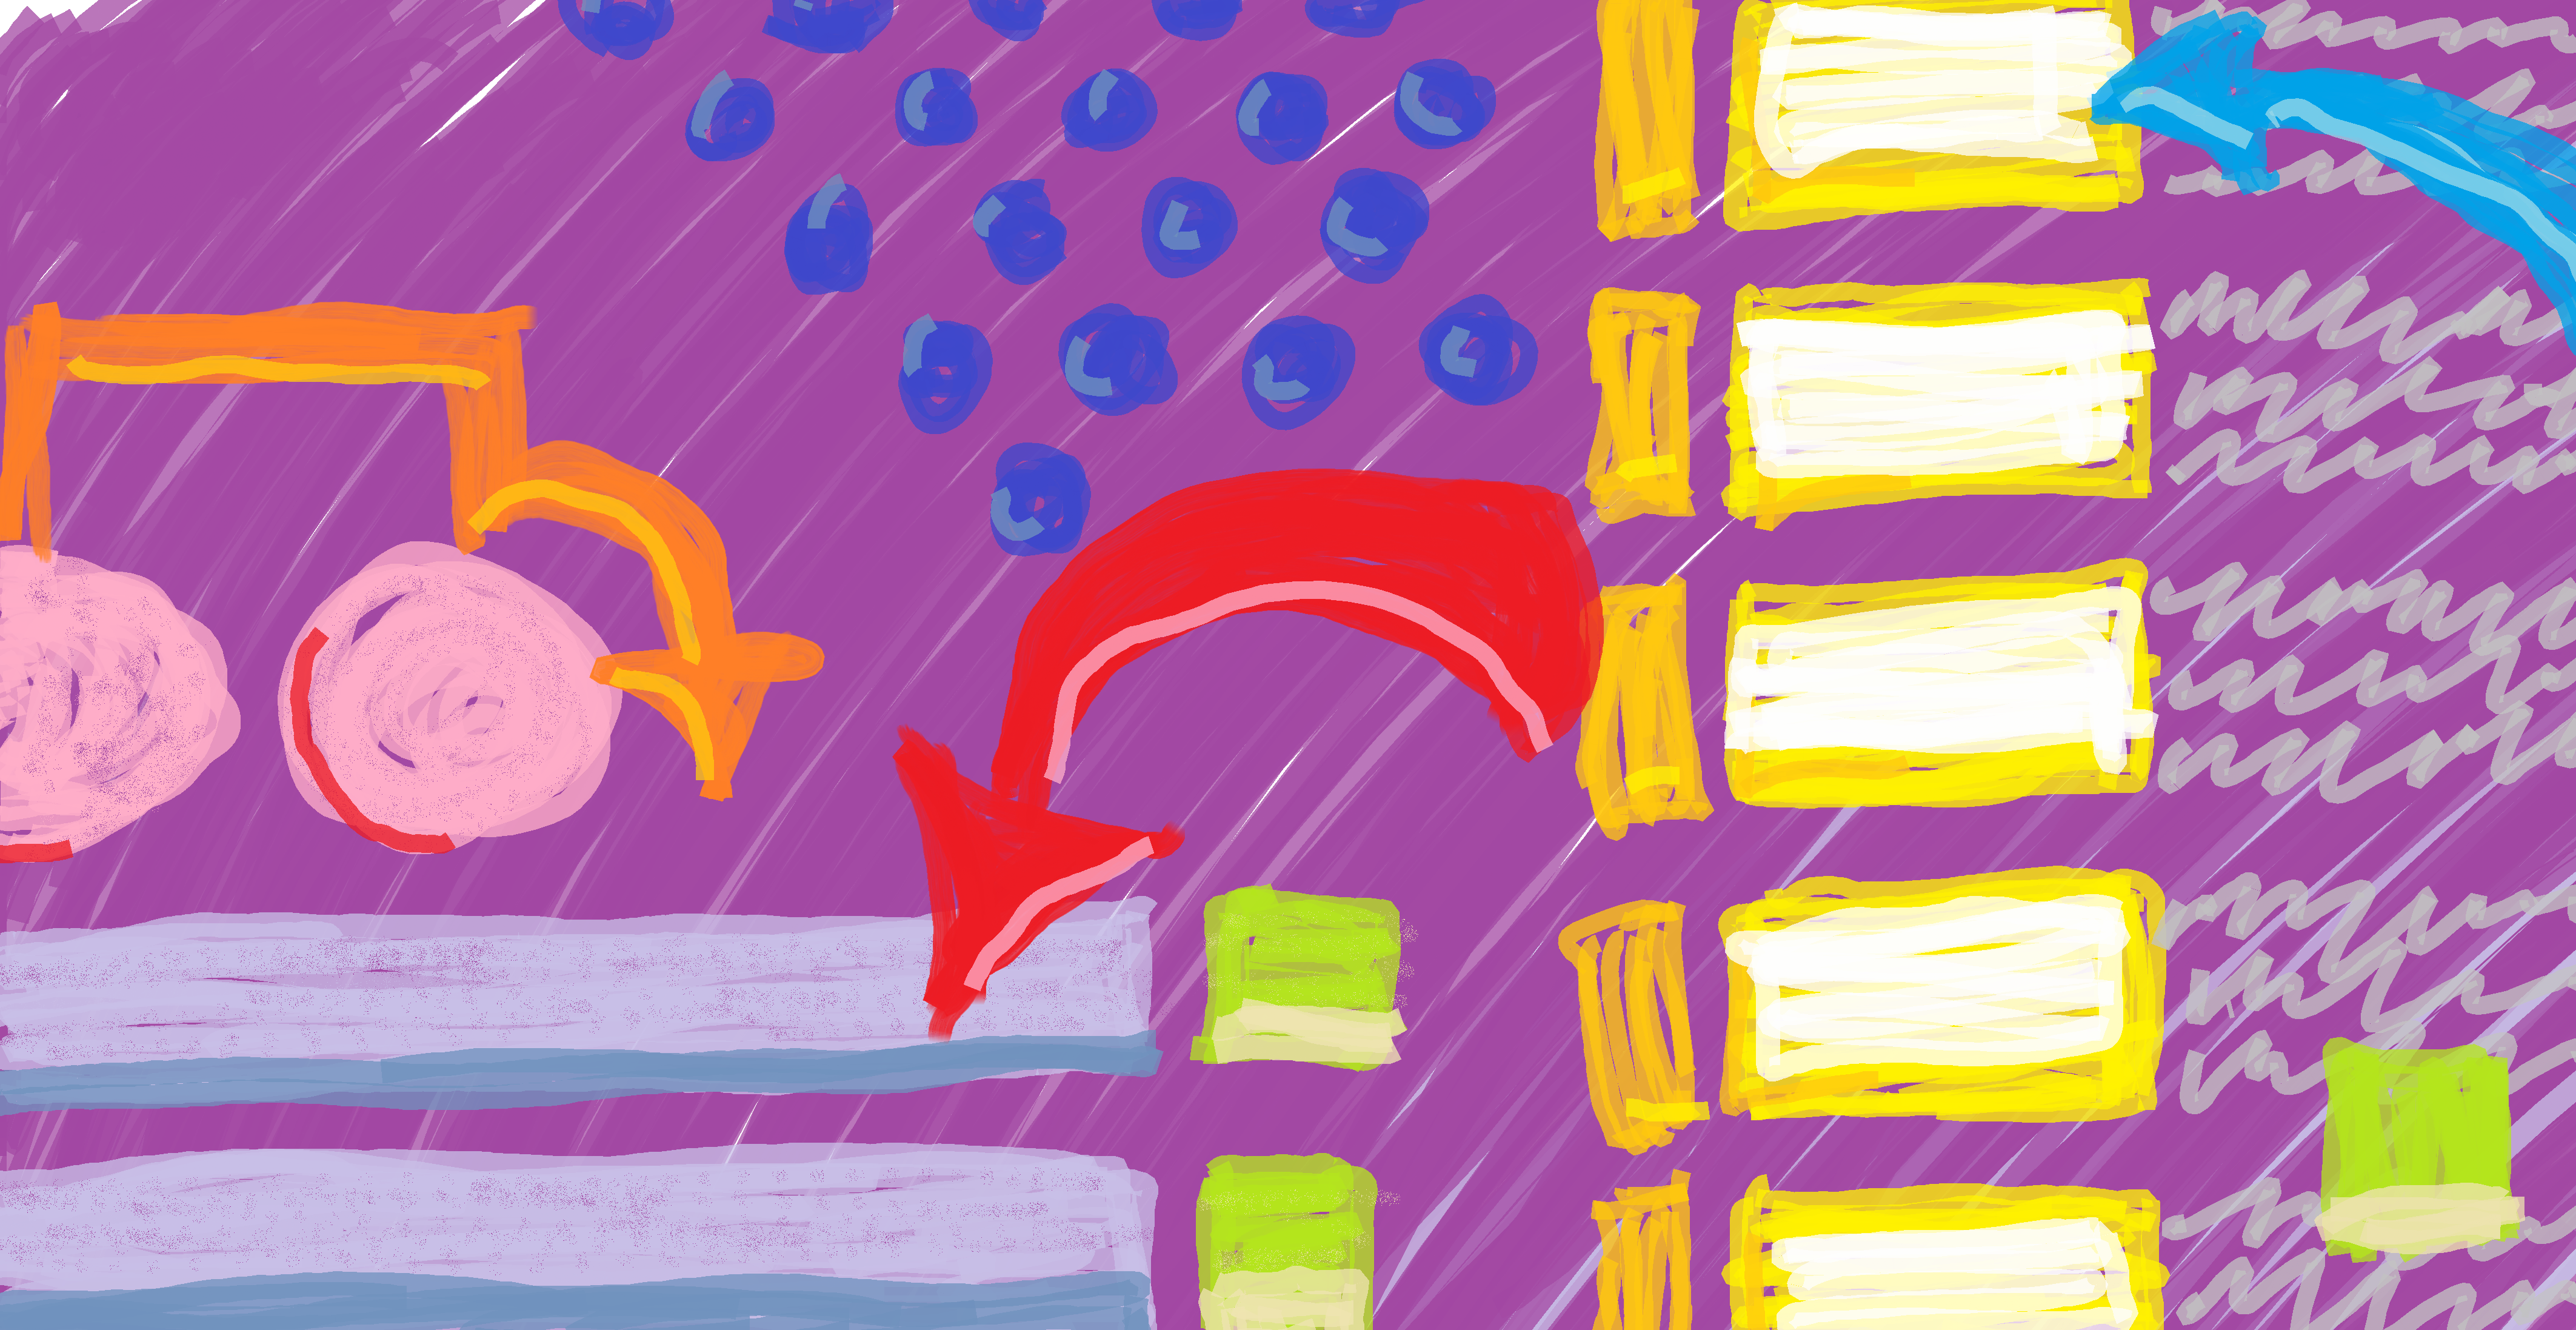
\includegraphics[width=9in]{pp}}; 
\end{tikzpicture} 

\marginpar{\userInterfaceDef}

\textbf{User interface}\index{user interface} (UI) design\index{user interface design} often involves prototyping\index{prototyping}: Iteratively creating depictions of what you think the UI\index{user interface} should look like, and how users should interact with it, based on the software's requirements\index{requirements}. \textbf{Prototyping}\index{prototyping} gives you a way to try out a UI\index{user interface} design\index{user interface design} and find problems early. Changing a drawing (digital or physical) is easier and faster than changing its code implementation.

There are multiple levels---or ``fidelities''\index{fidelity (of prototypes)}---of UI\index{user interface} design\index{user interface design} prototypes\index{prototyping} (low-fidelity\index{low-fidelity (prototype)}, medium-fidelity\index{medium-fidelity (prototype)}, and high-fidelity\index{high-fidelity (prototype)}). If you look around, you'll find disagreement on the definitions\index{fidelity (of prototypes)}. 
\textbf{Definitions I use:}

\begin{itemize}

\item{\textbf{Low-fidelity}: A rough sketch that is often drawn by hand, drawn using an app and stylus, or made using software specifically for creating low-fidelity prototypes. At this fidelity, you can \textbf{gather feedback on higher-level features} and have the \textbf{flexibility} to make large, low-cost changes.
\begin{center}
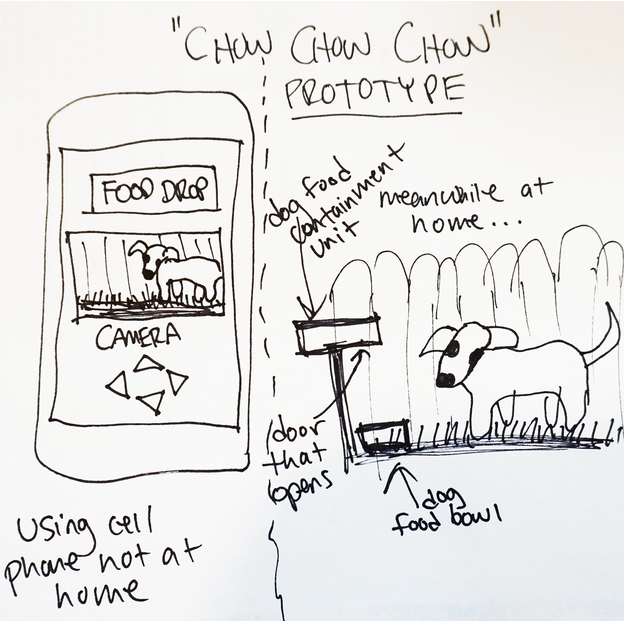
\includegraphics[width=3in]{uip-low-fidelity}
\end{center}\marginpar{\guiDef\margindivider}\marginpar{\lowFidelityPrototypeDef\margindivider}\marginpar{\mediumFidelityPrototypeDef}
\spacer
}
\item{\textbf{Medium-fidelity}: A \textbf{detailed} illustration often created using a professional drawing or presentation tool (e.g., Visio, PowerPoint, etc.), or perhaps a careful and detailed hand-drawing. At this fidelity, to keep costs low, you can gather feedback on \textbf{small changes} to defined and accepted features that you plan to keep but might change the look of.
\begin{center}
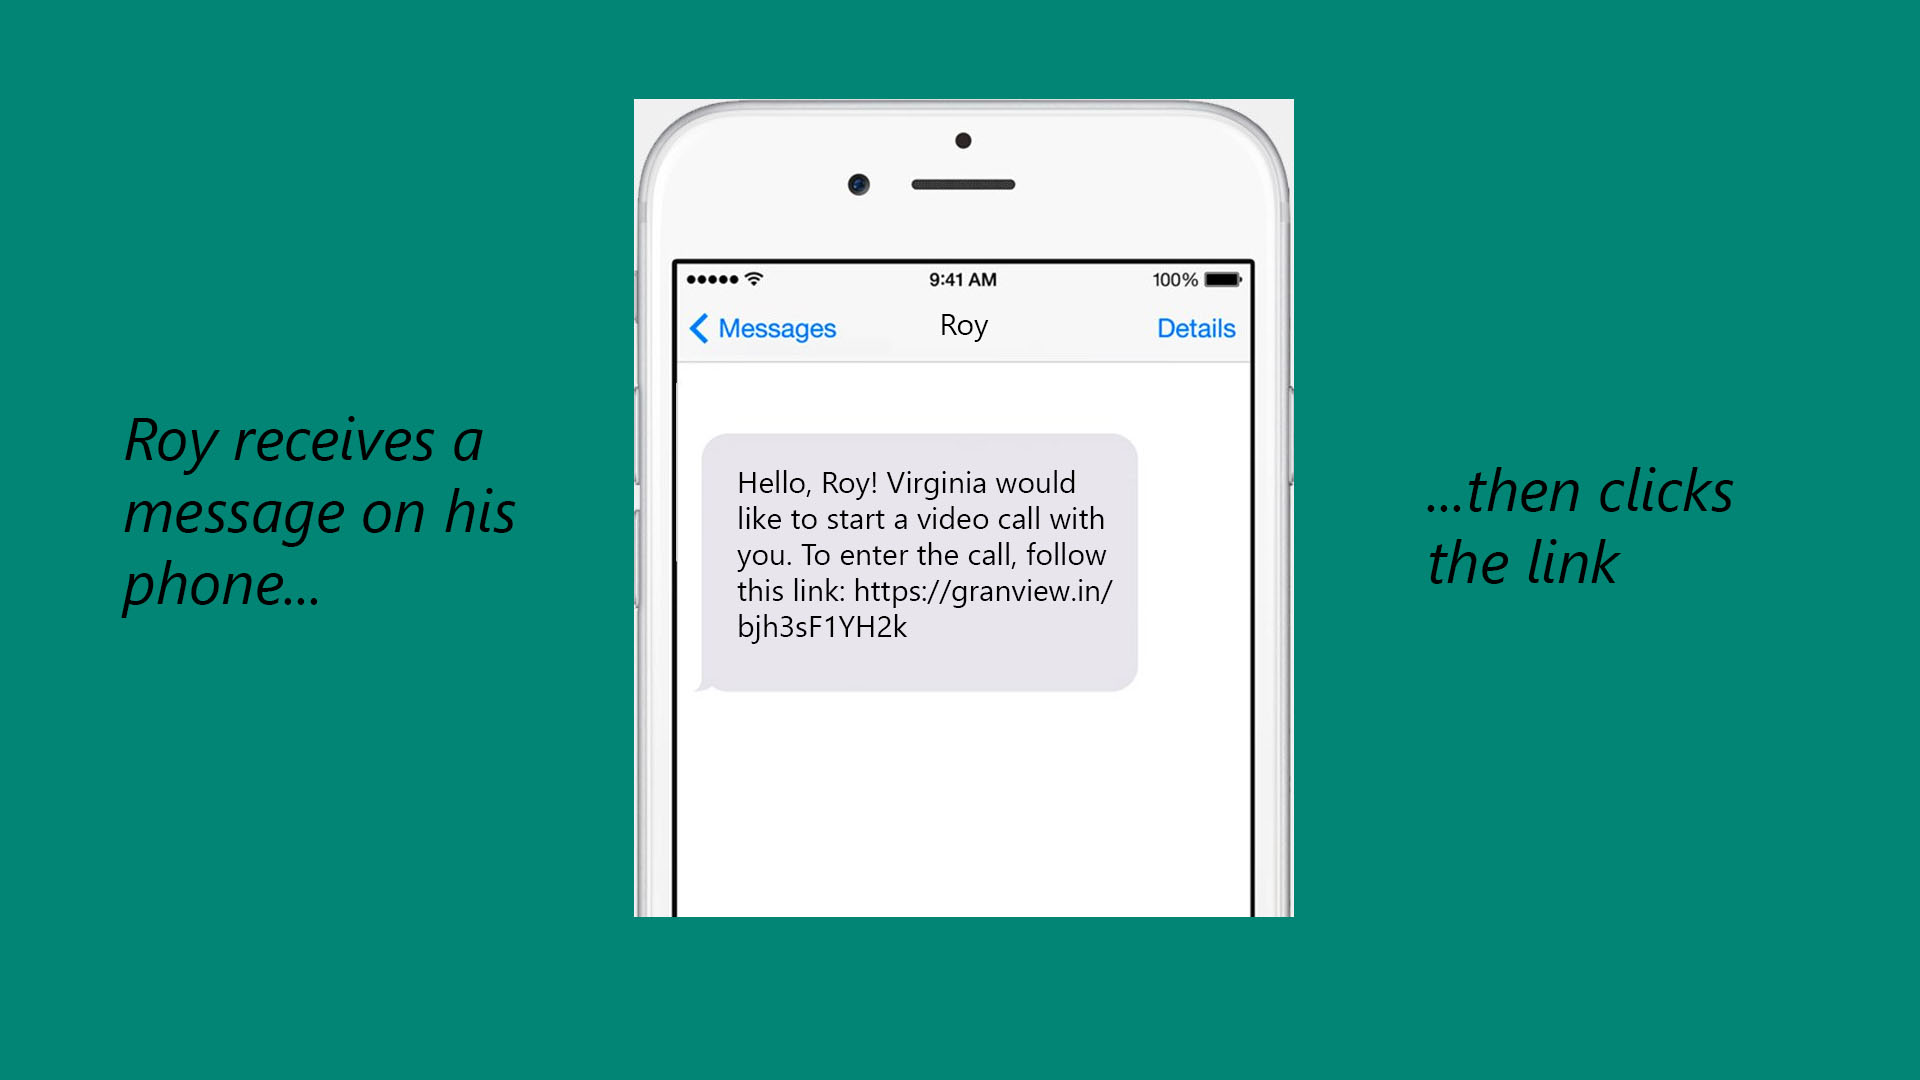
\includegraphics[width=\textwidth]{uip-medium-fidelity}
\end{center}
}

\item{\textbf{High-fidelity}: A \textbf{polished}, detailed illustration that looks like a finished UI. These designs might be created in a full-featured graphics editor (e.g., Photoshop, Illustrator, etc.) or a GUI builder. At this fidelity, to keep costs low, you can gather feedback about \textbf{detailed tweaks} to specific features to make very focused and incremental improvements.

\marginpar{\highFidelityPrototypeDef\margindivider}\marginpar{\paperPrototypeDef}
\begin{center}
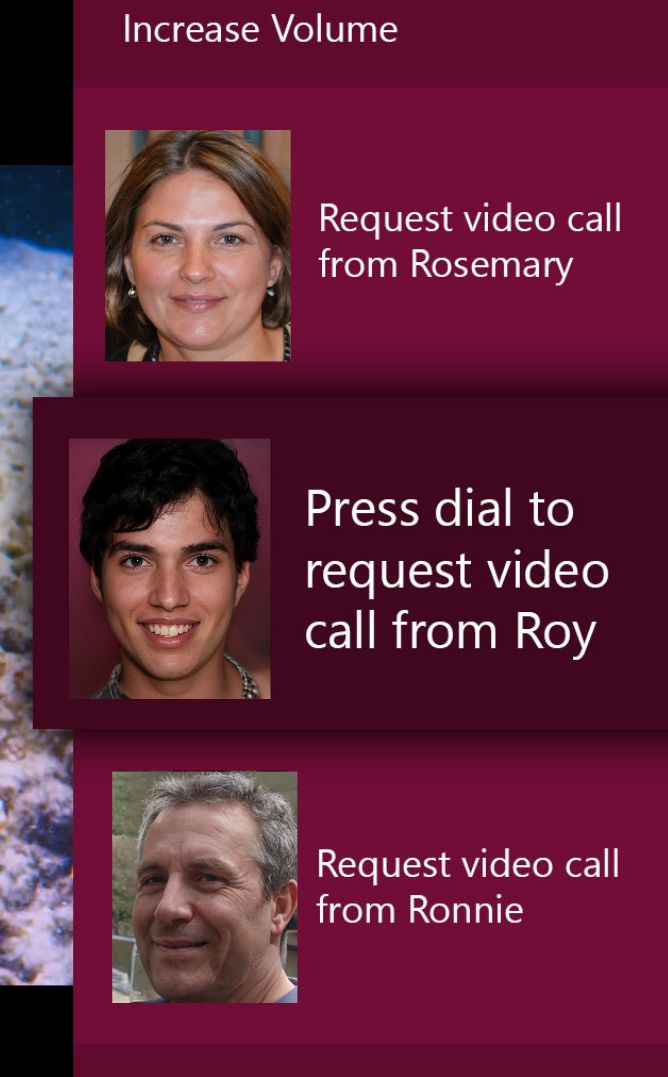
\includegraphics[width=2in]{uip-high-fidelity}
\end{center}
}
\end{itemize}

A quick and low-cost way to begin prototyping (and begin getting feedback on your UI design) is to create a low-fidelity \textbf{paper prototype}.

A paper prototype is a hand-drawn sketch of a UI design that's based on the software's requirements. It \textbf{does not need to be pretty or artistic}. It can be simple and reduce the UI to only the most important elements (i.e., it is often low-fidelity).

\section{Showing Interaction}

A paper prototype \textbf{needn't be static} or limited to one sheet of paper. With some craftiness and creativity, paper prototypes can communicate elements of \textbf{interaction design}\marginpar{\interactionDesignDef}\index{interaction design} by indicating what users can interact with (e.g., a slider), how they can interact (e.g., by dragging), and what happens when they interact (e.g., an overlay appears, showing the elevations of each mountain in the photo). To show interaction design through a paper prototype, you can, for example, cut out small paper shapes you can easily move around (e.g., a small rectangle showing the submenu items that appear when a user clicks), place arrows and annotations on your prototype, and even add strings to show how UI elements may move. I've even seen people use brass brads for spinnable elements. But keep in mind that, if your client doesn't like your design, you might have saved time and communicated your concept just as well with a less elaborate paper prototype.

\section{Showing Your Concept to Others}

\marginpar{\thinkAloudProtocolDef}Once you have a paper prototype, you can \textbf{use it to harvest feedback}. Here's one way: If each of your screen designs is on one piece of paper, give your user the entry screen drawing, then either give them an objective (e.g., submit data report) or let them explore on their own. Watch as they tap buttons or otherwise interact. Be ready to place other drawings on top of the one they have to indicate what would happen in the real software (e.g., if they tap the gear icon, give them a sketch of the settings screen). If you're fast and brought extra supplies, you can construct new designs on-the-fly or (if they're interested) let your user participate. 

You can ask your user to provide feedback about the design after they're done using it or as they go, using a \textbf{think-aloud protocol}: Ask your user to tell you what they're doing, what they're trying to do, what questions they have at that moment, what they don't like, etc.

\nomargins
\section{Conclusion}
Paper prototyping can help reduce project costs by giving a way to detect user interface design flaws before they are implemented. It can also help teams communicate about the software with each other, clients, and users.

\section{Additional Resources}

\begin{description}
\item \fullcite{lewis93}
\item \fullcite{norman13}
\item \fullcite{snyder03}
\end{description}